\documentclass[a4paper,  onecolumn]{IEEEtran} % onecolumn
%
\usepackage{subscript}
\usepackage[T1]{fontenc}
\usepackage[utf8]{inputenc}
\usepackage{amssymb}
\usepackage{graphicx}
\usepackage{pgf}
\usepackage{tikz}
\usetikzlibrary{arrows,shadows} % for pgf-umlsd
\usetikzlibrary{arrows,automata}
\usepackage{pgf-umlsd}
\usepackage{fancybox}
\usepackage{algorithm}
\usepackage{algorithmic}
\usepackage{listings}






\begin{document}


\title{Clusterung von Sensorknoten zur Waldbranddektion}

\author{
  \IEEEauthorblockN{Robert Oehlmann, Jan Winkelmann}
  \IEEEauthorblockA{\\Hamburg University of Technology\\
    Institute of Communication Networks\\
  }
}

\maketitle

%\begin{abstract}
%  \boldmath
%  abstract goes here

%\\end{abstract}

\IEEEpeerreviewmaketitle
\IEEEoverridecommandlockouts

\section{Einleitung} \label{sec:intro}
\IEEEPARstart{D}{ieser} Bericht dokumentiert ein Protokoll zur Bildung von Clustern aus Sensorknoten um Strom zu sparen. Innerhalb der Cluster wird kein Routing ben\"otigt, und jedes Mitglied des Clusters kann die Verwaltungsaufgaben \"ubernehmen.

Wir beginnen mit einer weiterf\"uhrenden Beschreibung des Anwendungsszenarios und den getroffenen Annahmen in Abschnitt \ref{sec:setting}.
Darauf folgt Abschnitt \ref{sec:features} mit der Spezifikation der funktionalen Anforderungen.
Abschnitt \ref{sec:algo} besch\"aftigt behandelt das entwickelte Protokoll.
In Abschnitt \ref{sec:impl} wird die Implementierung der Simulation erläutert und anschließend in Abschnitt \ref{sec:ana} mit Bezug auf die funktionalen Anforderungen analysiert.


Als letztes werden in Abschnit \ref{sec:futwork} Ans\"atze f\"ur zuk\"unftige Arbeit erw\"ahnt, und in Abschnitt \ref{sec:conclusion} ein Fazit gezogen.

\section{Setting} \label{sec:setting}
Dieser Abschnitt beschreibt zuerst das Anwendungsgebiet, und danach die Annahmen die bei dem Design des Protokolles gemacht wurden.
W\"ahrend des Entwerfens des Protokolles, wurde nicht drauf geachtet das Anwendungszenario realistisch zu gestalten. Weder das Anwendungsszenarion noch Annahmen beruhen auf recherchierten Fakten.

\subsection{Anwendungsgebiet}
Um Fr\"uhwarnsysteme f\"ur Waldbr\"ande zu verbessern k\"onnten z.B. kleine Sensoren eingesetzt werden, welche sich untereinander vernetzen um so gro\ss e Fl\"achen messen zu k\"onnen.
In unserem Szenario seien Sensoren gegeben, die neben dem Messen von Metriken die f\"ur die Waldbranderkennung n\"otig sind, auch \"uber zwei Kommunikationsmethoden verf\"ugen. Eine Kommunikationsm\"oglichkeit zur Verst\"andigung mit anderen Sensoren in der unmittelbaren Umgebung, wie zum Beispiel W-LAN, und eine zum Senden der Messergebnisse an eine Senke, wie zum Beispiel GPRS.

Ziel dieses Projektes es nun, Sensorknoten in \emph{Cluster} zu organisieren.
Cluster benuzten Kurzstrecken-Kommunikation um den Sensoren zu erm\"oglichen Energie zu sparen, indem die Messdaten bei manchen Sensoren gesammelt werden, und so nicht jeder Sensor seine Daten einzeln zu der Senke senden muss.
Die Sensoren, welche die Messdaten zur Senke sendet bezeichnen wir als \emph{Clusterhead}.

\subsection{Annahmen}
Die technischen Voraussetzungen f\"ur unseren Ansatz sind die Folgenden:
\begin{itemize}
\item Alle Sensorknoten sind baugleich, d.h. jeder Sensorknoten kann mit anderen Sensorknoten und der Senke kommunizieren.
\item Keine zwei Sensorknoten versuchen gleichzeitig einem Cluster beizutreten. Dies wird  dadurch erreicht, dass alle  Sensorknoten sich nacheinander aktivieren.
\item Sensorknoten bewegen sich nicht.
\item Keine Ausfälle von einzelnen Verbindungen. Ein Sensorknoten erreicht entweder alle Knoten seines Clusters, oder keine.
\item Keine tempor\"aren Ausf\"alle. Ein Sensorknoten f\"allt entweder nicht oder komplett aus.
\item Wenn ein Sensorknoten ausf\"allt, so merken es alle Sensorknoten im Cluster gleichzeitig und mit Sicherheit, aber nicht zwingend instantan.
\end{itemize}

\noindent Zus\"atzlich nehmen wir an, dass ein unterliegendes Protokoll existiert, das folgendes garantiert:
\begin{itemize}
\item Garantierte Zustellung von Nachrichten
\item Zustellung der Nachrichten in der richtigen Reihenfolge
\end{itemize}
Ein Beispiel hierf\"ur w\"are ein TCP/IP Stack.

\section{Funktionale Anforderungen} \label{sec:func}
\begin{enumerate}
\item \textbf{Clusterbildung nach dem beschriebenen Protokoll}
  \begin{itemize}
  \item \emph{Beschreibung:}\\
    Die Implementation hat aus Mote-Objekten Cluster zu bilden. Die Bildung der Cluster hat nach dem in Abschnitt \ref{sec:algo} beschriebenen Algorithmus zu erfolgen.
  \item \emph{Problembeschreibung:}\\
    Prim\"ares Ziel des Projektes ist das Bilden von Clustern von Sensorknoten. Die Wichtigkeit dieses Punktes ist daher \emph{kritisch} und selbsterkl\"arend.
  \item \emph{Abnahmekriterium:}\\
    Diese Anforderung gelte als erf\"ullt, sobald die Mote-Objekte der Implementation bereitstellt, die das Protokoll zur Formung von Clustern vollst\"andig implementieren.
  \end{itemize}
\item \textbf{Rotation des Clusterheads nach dem beschriebenen Protokoll}
  \begin{itemize}
  \item \emph{Beschreibung:}\\
    Die durch Punkt 1 gebildeten Cluster haben einen Clusterhead. Die Implementation hat den Algorithmus zur Rotation der Clusterheads, welcher auch in Abschnitt \ref{sec:algo} beschrieben ist, zu implementieren.
  \item \emph{Problembeschreibung:}\\
    Eine der Priorit\"aten bei dem Design des Protokolles zum Bilden von Clustern war die Austauschbarkeit der Clusterheads. Durch die Reduktion auf vollst\"andige Graphen ist die einfach zu erreichen. Die Rotation ist daher ein guter Showcase f\"ur die Vorz\"uge des Protokolls zum Bilden von Clustern.
  \item \emph{Abnahmekriterium:}\\
    Diese Anforderung gelte als erf\"ullt, wenn die gebildeten Cluster den Clusterhead nach dem spezifizierten Protokoll implentiert.
  \end{itemize}
\item \textbf{Kapselung der Komponenten}
  \begin{itemize}
  \item \emph{Beschreibung:}\\
    Einzelne Systemkomponenten haben auf realistische Weise voneinander gekapselt sein.
    Dies bezieht sich insbesondere, aber nicht aussschlie\ss lich auf den Motes zur Verf\"ugung stehenden Informationen, wie Lage, Informationen \"uber andere Sensorknoten, sowie Zustellung der Kommunikationen unter dem Motes durch einen von dem Sensorknoten unabh\"anigen Mechanismus.
  \item \emph{Problembeschreibung:}\\
Um eine m\"oglichst realistische Simulation zu sein, und um als echter Proof-Of-Concept zu gelten, m\"ussen die simulierten Komponenten voneinander entkoppelt sein, also \"uber Schnittstellen kommunizieren, welche auch in einem Anwendungszenarion bestehen w\"urden.
  \item \emph{Abnahmekriterium:}\\
    Zur Erf\"ullung dieser Anforderung sind n\"otig: Kapselung der Mote-Objekte untereinander, Kapselung der Mote-Objekte von der Simulationsumgebung und ein Mechanismus zum Nachrichtenversenden.
  \end{itemize}
\item \textbf{Graphische Oberfl\"ache}
  \begin{itemize}
  \item \emph{Beschreibung:}\\
    Die Implementation hat eine graphische Benuzteroberfl\"ache zur Verf\"ugung zu stellen, welche die Simulation visualisiert. Die Bedienung der Oberfl\"ache hat ein sinnvolles Subset der Gesamtfunkionalit\"at zu implementieren.
  \item \emph{Problembeschreibung:}\\
    Um die Simulation zu visualisieren ist eine graphische Oberfl\"ache unentbehrlich. Sie dient zur demonstration des Proof-Of-Concepts. Das Hinzuf\"ugen und Entfernen von Motes erlaubt das Demonstrieren des vollen Umfanges der Funktionalit\"at.
  \item \emph{Abnahmekriterium:}\\
    Die Implementation muss eine graphische Benuzteroberfl\"ache haben, welche die simulierte Umgebung, samt Sensoreknoten darstellt. Gebildete Cluster m\"ussen farblich markiert sein. Zus\"atzlich soll man Sensorknoten hinzuf\"ugen und entfernen k\"onnen.
  \end{itemize}
\item \textbf{Ausfallsicherheit?}
\end{enumerate}

\section{Protokoll} \label{sec:algo}
Dieser Abschnitt besch\"aftigt sich mit den entwickelten Algorithmen f\"ur das bilden von Clustern, die Ausfallsicherheit, und das Rotieren von Clusterheads.

\subsection{Clusterbildung}
Die Grundlage des Bildes von Clustern ist das Finden von vollst\"andigen Sub-Graphen.
Die Knoten des Graphen sind die Sensorknoten, und die Kanten die Verbindungen zu anderen Sensorknoten in Reichweite.
Dadurch reduziert sich die Clusterbildung auf das Cliquenproblem, ist aber aufgrund der getroffenen Annahmen nicht in $NP$.

Sensorknoten ordnen sich nach der Aktivierung einem Cluster zu, und verlassen diesen nicht, bis der Cluster sich aufl\"ost. Es werden keine Optimierungen an bestehenden Clustern vorgenommen.
Siehe Bild \ref{fig:sm} f\"ur die Finite-State-Machine des Protokolls.

Cluster werden durch folgendes Protokol gebildet:
\begin{enumerate}
\item Falls sich ein Sensor aktiviert, so sendet sie zuerst eine Nachricht die nach vorhandenen Clustern sucht. Findest der Sensor keine vorhandenen Cluster, so bildet er selber einen.
\item Alle schon vorhandenen Clusterheads antworten auf die Anfragen von neuen Knotens. Diese Antwort enth\"allt einen Identifikator des Clusters und die Anzahl der Sensoren in dem Cluster.
\item Der neue Sensor speichert alle Antworten der vorhanden Cluster, ordnet sie nach Gr\"o\ss e und versucht der Reihe nach einem der Cluster beizutreten, beginnend mit dem Kleinsten.
\item Der erste Schritt zum Beitreten eines Clusters, das Senden eine Nachricht, auf die alle Mitglieder des Clusters mit ihrer Id antworten.
\item Nach dem Ablaufen eines Timeouts, sendet der neue Sensor die Ids aller empfangenen Sensoren an den Clusterhead. Dies stellt sicher, dass der neue Sensor alle schon vorhandenen Mitglieder erreichen kann.
\item Falls die Nachricht des neuen Sensors alle Ids des aktuellen Clusters entahlten, so sendet der Clusterhead dem neuen Sensor eine Nachricht mit der Best\"atigung, dass er neue Sensor dem Cluster beigetreten ist. Zus\"atzlich ordnet der Clusterhead dem neuen Sensor einen Slot zu. Dieser Slot wird n\"otig, falls der Clusterhead ausf\"allt.
\item Falls die Nachricht des neuen Sensors nicht alle Ids enthalten sollte, so sendet der Server eine Ablehnung und der Client versucht dem n\"achst gr\"o\ss eren Cluster beizutreten.
\end{enumerate}
Bild \ref{fig:sd} ist ein UML-Sequenzdiagram welches einen erfolgreichen Clusterbeitritt mit einem weiterem Sensorknoten illustiert.


\begin{figure*}
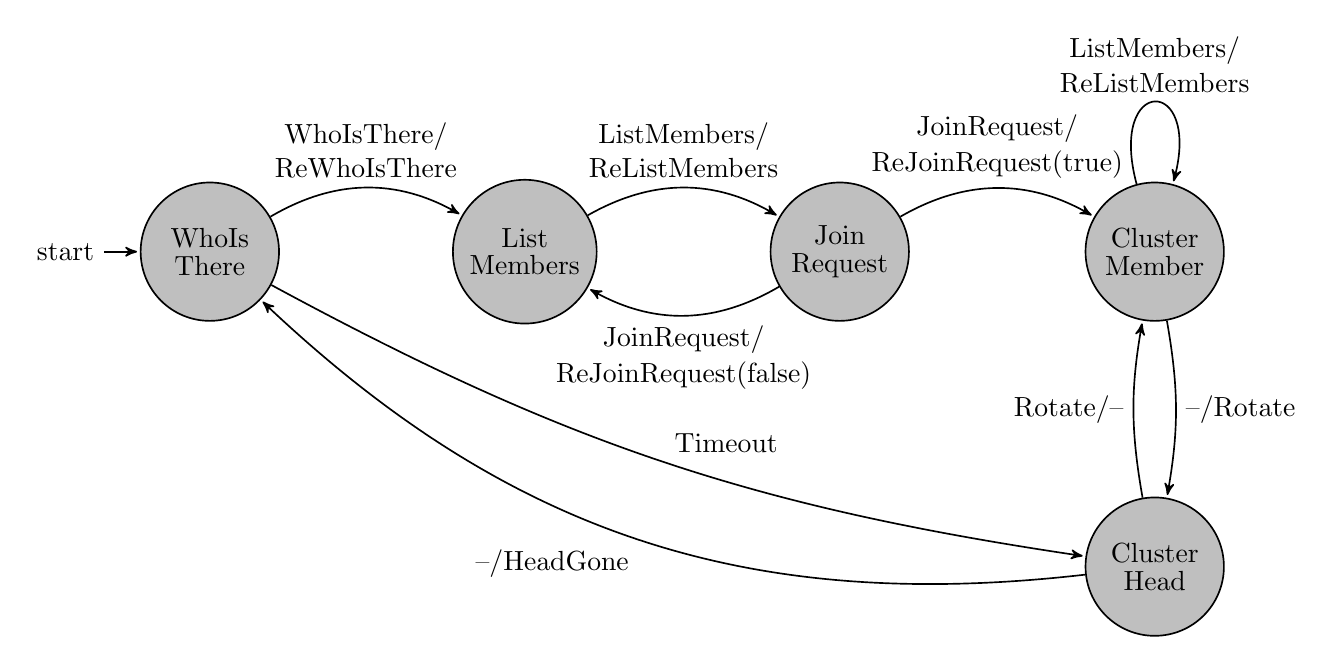
\begin{tikzpicture}[->,>=stealth',shorten >=1pt,auto,node distance=4cm,
                    semithick]
  \tikzstyle{every state}=[circle,fill=black!25, minimum size=5em]

  \node[initial,state] (A)              {\shortstack{WhoIs\\There}};
  \node[state]         (B) [right of=A] {\shortstack{List\\Members}};
  \node[state]         (C) [right of=B] {\shortstack{Join\\Request}};
  \node[state]         (D) [right of=C] {\shortstack{Cluster\\Member}};
  \node[state]         (E) [below of=D] {\shortstack{Cluster\\Head}};

  \path (A) edge [bend right=10]  node {Timeout} (E)
            edge [bend left]  node {\shortstack{WhoIsThere/\\ReWhoIsThere}} (B)
        (B) edge [bend left]  node {\shortstack{ListMembers/\\ReListMembers}} (C)
        (C) edge [bend left]  node {\shortstack{JoinRequest/\\ReJoinRequest(true)}} (D)
            edge [bend left] node {\shortstack{JoinRequest/\\ReJoinRequest(false)}} (B)
        (D) edge [loop above] node {\shortstack{ListMembers/\\ReListMembers}} (D)
            edge [bend left=10]  node {--/Rotate} (E)
        (E) edge [bend left=10]  node {Rotate/--} (D)
            edge [bend left=25] node {--/HeadGone} (A);
\end{tikzpicture}
\label{fig:sm}
\caption{State Machine des Cluster Protokolls}
\end{figure*}

\begin{figure*}
  \centering
  \begin{sequencediagram}
    \tikzstyle{inststyle}+=[node distance=2.0cm] % custom the style
    \newthread{ch}{ClusterHead}
    \newthread{new}{New Mote}
    \newthread{cm}{ClusterMote}

    \begin{sdblock}{Join}{}
      \begin{call}{new}{WhoIsThere}{ch}{ReWhoIsThere}
      \end{call}

      \begin{call}{new}{ListMembers}{cm}{ReListMembers}
      \end{call}

      \begin{call}{new}{Join}{ch}{ReJoin}
      \end{call}
    \end{sdblock}


  \end{sequencediagram}
  \caption{Sequenzdiagram f\"ur einen erfolgreichen Clusterbeitritt}
  \label{fig:sd}
\end{figure*}

\subsection{Ausfallsicherheit}
Aufgrund der erw\"ahnten Annahmen (TCP/IP, keine Bewegung der Sensorknoten, etc) gibt es nur zwei Ausfallszenarien die betrachtet werden m\"ussen, der Ausfall des Clusterheads, sowie der Ausfall eines Sensorknotens der normales Mitglied in einem Cluster ist.
Falls ein normaler Sensorknoten ausfallen sollte, so muss der zugeh\"orige Clusterhead dies merken und die Liste der zum Cluster zugeh\"origen Sensorknoten aktualisieren.
Da Sensorkntoen die dem Cluster betreten wollen Kontakt zu allen Sensorknoten nachweisen m\"ussen, die der Cluster als zum Cluster zugeh\"orig gespeichert hat, w\"urde der unbemerkte Ausfall eines Sensorknotens dazu f\"uhren, dass keine neuen Knoten beitreten k\"onnen.
In einem realen Szenario erkennt der Clusterhead das Ausfallen eines normalen Knotens an dem Fehler von gesendeten Sensordaten. In der nie vorgestellten Simulation wird durch das L\"oschen direkt beim Server ein L\"oschevent.

Der Ausfall von einem Clusterhead wird durch das Fehlen von Best\"atigungsnachrichten erkannt.
Aufgrund unserer Annahme geschickt dies bei allen Knoten im Cluster gleichzeitig.
Sobald ein Knoten den Ausfall des Clusterheads wahrnimmt, so wird der Cluster als tot angenommen.
Der Knoten wartet nun eine bestimmte Zeit $b$ und versucht dann einem neuen Cluster beizutreten.
$b$ berechnet sich durch die upper bound f\"ur das Beitreten eines Sensorknoten zu einem Cluster multipliziert mit dem ``slot'' welcher dem Knoten beim Beitreten des jetzt toten Clusters zugewiesen wurde.
Der Slot ist ein streng monoton ansteigender, pro Cluster eindeutiger Integer.
Somit wird sichergestellt, dass die Knoten alle nacheinander in der urspr\"unglichen Beitrittsreihenfolge versuchen einem neuen Cluster beizutreten.

\subsection{Rotation der Clusterheads}
Die Rotation des Clusterhead ist der Prozess welcher von dem aktuellen Clusterhead ausgef\"uhrt wird, und einem anderen Knoten die F\"uhrung des Clusters zuweist.
Dieser Rotation kann ausgel\"ost werden von z.B. einem timeout oder dem Batteriestand.
Beider Durchf\"uhrung der Rotation w\"ahlst der Clusterhead der neuen Cluster und sickt alle relevanten Daten an ihn.
Die gesendeten Daten sind:
Der Slot der als n\"achstes vergeben wird, eine Liste der Ids aller Knoten in dem Cluster, sowie die Id des Clusters.

\section{Implementierung}

Um die dargelegten Algorithmen zu testen und zu demonstrieren, haben wir
eine Simulation entwickelt. Im folgenden wird zunächst die gewählte
Entwicklungsplattform vorgestellt und begründet, anschließend werden die
Implementierung des Äthers, der Motes und die Spezifika der
Simulations-Umgebung dargestellt.

\subsection{JavaScript}

Die Simulation ist in JavaScript implementiert; als
Entwicklungsplattform haben wir Webbrowser mit aktueller
JavaScript-Engine (z.B. Googles V8 und Mozillas JägerMonkey) und
Unterstützung für 2D-Grafikdarstellung mithilfe des canvas-Tags gewählt.

Mit JavaScript als dynamisch-typisierte Skriptsprache lassen sich ohne
große Deklartions-Overhead schnell sichtbare Ergebnisse produzieren. Mit
dem neuen HTML5 Canvas Element steht eine einfach zu nutzende
Zeichenfläche zur Verfügung und für alle gängigem Betriebssysteme gibt
es Browser die die Simulation auführen können.

\subsection{Motes}

Die simulierten Motes sind Instanze der Klasse Mote, deren
Implementierung sich über die Dateien mote.js, mote\_member.js und
mote\_head.js erstreckt.

Das in Abschnitt ?? dargestellte Protokoll ist vollständig, aber
zustandslos, in der Klasse Mote implememtiert.

Wird eine neue Mote instanziert, initialisiert der Konstruktur einige
interne Variablen, registriert die neue Mote dann beim Äther und kann
dann gestartet (``eingeschaltet'') werden.

\subsection{Äther}

Die Motes kommunizieren untereinander nur über Nachrichten. Den
(virtuellen) Versandt der Nachrichten übernimmt der simulierte Äther,
implementiert als Singleton ``MoteList'' in der Datei motelist.js.

Ähnlich dem Observer-Entwurfsmuster stellt MoteList eine Methode
``register'' bereit, die neuer Motes aufnimmt. Sie wird vom
Mote-Konstruktur aufgerufen. Zudem gibt es eine Methode ``send'', die
den Versandt von Nachrichten anstößt.

Beim Versandt wird zunächst die Position des Absenders abgerufen,
anschließend wird die Distanz zu allen anderen registrierten Motes
berechnet. Ist die Distanz nicht größer als ein festgelegter
Senderadius, wird die Nachricht zugestellt indem sie der ``onRecv''
Methode der jeweiligen Empfänger-Mote übergeben wird.

\subsection{Grafische Oberfläche}

Die grafische Oberfläche beschränkt sich im wesentlichen auf eine
``Karte'' in der alle Motes, möglichen Verbindungen, sowie Cluster
verzeichnet sind.

Die Zeichenfunktion ist dabei in der MoteList implementiert, da nur
diese Zugriff auf die Positionen der Motes hat.

Die Motes sind als kleine Quadrate auf der Karte dargestellt, oberhalb
eines Cluser-Heads wird jeweils die ID des Clusters angezeigt. Zwischen
Motes die nicht mehr als einen Senderadius voneinander entfernt sind,
ist eine blasse Linie eingezeichnet. Zwischen zwei Motes die zu einem
Cluster gehören, wird diese Linie farblich hervorgehoben.

Weitere Motes werden hinzugefügt, wenn man auf eine freie Fläche der
Karte klickt. Klickt man eine vorhandene Mote an, wird diese entfernt.

Die Rotation der Cluster-Heads wird durch Drücken der Taste 'r'
angestoßen. Die Taste 'a' schaltet eine automatische Rotation der
Cluster-Heads in einem fixen Intervall ein oder aus.

\section{Analyse} \label{sec:ana}
Robert... (This is also a placeholder)



\section{Future Work} \label{sec:fut}
Jan will write about future work here.
Jan will write about:\\
Mehr als eine neue Moye gleichzeitig\\
implementation als fsm\\
ausfall von kanten\\
cluster regroupen\\
realitaetsnaehe abchecken mit bestehenden wifi protokollen\\

\section{Lessons Learned} \label{sec:les}
??


\end{document}
